% Options for packages loaded elsewhere
\PassOptionsToPackage{unicode}{hyperref}
\PassOptionsToPackage{hyphens}{url}
\PassOptionsToPackage{dvipsnames,svgnames,x11names}{xcolor}
%
\documentclass[
  letterpaper,
  DIV=11,
  numbers=noendperiod]{scrartcl}

\usepackage{amsmath,amssymb}
\usepackage{iftex}
\ifPDFTeX
  \usepackage[T1]{fontenc}
  \usepackage[utf8]{inputenc}
  \usepackage{textcomp} % provide euro and other symbols
\else % if luatex or xetex
  \usepackage{unicode-math}
  \defaultfontfeatures{Scale=MatchLowercase}
  \defaultfontfeatures[\rmfamily]{Ligatures=TeX,Scale=1}
\fi
\usepackage{lmodern}
\ifPDFTeX\else  
    % xetex/luatex font selection
\fi
% Use upquote if available, for straight quotes in verbatim environments
\IfFileExists{upquote.sty}{\usepackage{upquote}}{}
\IfFileExists{microtype.sty}{% use microtype if available
  \usepackage[]{microtype}
  \UseMicrotypeSet[protrusion]{basicmath} % disable protrusion for tt fonts
}{}
\makeatletter
\@ifundefined{KOMAClassName}{% if non-KOMA class
  \IfFileExists{parskip.sty}{%
    \usepackage{parskip}
  }{% else
    \setlength{\parindent}{0pt}
    \setlength{\parskip}{6pt plus 2pt minus 1pt}}
}{% if KOMA class
  \KOMAoptions{parskip=half}}
\makeatother
\usepackage{xcolor}
\usepackage[top=15mm, bottom=15mm, left=15mm, right=15mm]{geometry}
\setlength{\emergencystretch}{3em} % prevent overfull lines
\setcounter{secnumdepth}{-\maxdimen} % remove section numbering
% Make \paragraph and \subparagraph free-standing
\ifx\paragraph\undefined\else
  \let\oldparagraph\paragraph
  \renewcommand{\paragraph}[1]{\oldparagraph{#1}\mbox{}}
\fi
\ifx\subparagraph\undefined\else
  \let\oldsubparagraph\subparagraph
  \renewcommand{\subparagraph}[1]{\oldsubparagraph{#1}\mbox{}}
\fi

\usepackage{color}
\usepackage{fancyvrb}
\newcommand{\VerbBar}{|}
\newcommand{\VERB}{\Verb[commandchars=\\\{\}]}
\DefineVerbatimEnvironment{Highlighting}{Verbatim}{commandchars=\\\{\}}
% Add ',fontsize=\small' for more characters per line
\usepackage{framed}
\definecolor{shadecolor}{RGB}{241,243,245}
\newenvironment{Shaded}{\begin{snugshade}}{\end{snugshade}}
\newcommand{\AlertTok}[1]{\textcolor[rgb]{0.68,0.00,0.00}{#1}}
\newcommand{\AnnotationTok}[1]{\textcolor[rgb]{0.37,0.37,0.37}{#1}}
\newcommand{\AttributeTok}[1]{\textcolor[rgb]{0.40,0.45,0.13}{#1}}
\newcommand{\BaseNTok}[1]{\textcolor[rgb]{0.68,0.00,0.00}{#1}}
\newcommand{\BuiltInTok}[1]{\textcolor[rgb]{0.00,0.23,0.31}{#1}}
\newcommand{\CharTok}[1]{\textcolor[rgb]{0.13,0.47,0.30}{#1}}
\newcommand{\CommentTok}[1]{\textcolor[rgb]{0.37,0.37,0.37}{#1}}
\newcommand{\CommentVarTok}[1]{\textcolor[rgb]{0.37,0.37,0.37}{\textit{#1}}}
\newcommand{\ConstantTok}[1]{\textcolor[rgb]{0.56,0.35,0.01}{#1}}
\newcommand{\ControlFlowTok}[1]{\textcolor[rgb]{0.00,0.23,0.31}{#1}}
\newcommand{\DataTypeTok}[1]{\textcolor[rgb]{0.68,0.00,0.00}{#1}}
\newcommand{\DecValTok}[1]{\textcolor[rgb]{0.68,0.00,0.00}{#1}}
\newcommand{\DocumentationTok}[1]{\textcolor[rgb]{0.37,0.37,0.37}{\textit{#1}}}
\newcommand{\ErrorTok}[1]{\textcolor[rgb]{0.68,0.00,0.00}{#1}}
\newcommand{\ExtensionTok}[1]{\textcolor[rgb]{0.00,0.23,0.31}{#1}}
\newcommand{\FloatTok}[1]{\textcolor[rgb]{0.68,0.00,0.00}{#1}}
\newcommand{\FunctionTok}[1]{\textcolor[rgb]{0.28,0.35,0.67}{#1}}
\newcommand{\ImportTok}[1]{\textcolor[rgb]{0.00,0.46,0.62}{#1}}
\newcommand{\InformationTok}[1]{\textcolor[rgb]{0.37,0.37,0.37}{#1}}
\newcommand{\KeywordTok}[1]{\textcolor[rgb]{0.00,0.23,0.31}{#1}}
\newcommand{\NormalTok}[1]{\textcolor[rgb]{0.00,0.23,0.31}{#1}}
\newcommand{\OperatorTok}[1]{\textcolor[rgb]{0.37,0.37,0.37}{#1}}
\newcommand{\OtherTok}[1]{\textcolor[rgb]{0.00,0.23,0.31}{#1}}
\newcommand{\PreprocessorTok}[1]{\textcolor[rgb]{0.68,0.00,0.00}{#1}}
\newcommand{\RegionMarkerTok}[1]{\textcolor[rgb]{0.00,0.23,0.31}{#1}}
\newcommand{\SpecialCharTok}[1]{\textcolor[rgb]{0.37,0.37,0.37}{#1}}
\newcommand{\SpecialStringTok}[1]{\textcolor[rgb]{0.13,0.47,0.30}{#1}}
\newcommand{\StringTok}[1]{\textcolor[rgb]{0.13,0.47,0.30}{#1}}
\newcommand{\VariableTok}[1]{\textcolor[rgb]{0.07,0.07,0.07}{#1}}
\newcommand{\VerbatimStringTok}[1]{\textcolor[rgb]{0.13,0.47,0.30}{#1}}
\newcommand{\WarningTok}[1]{\textcolor[rgb]{0.37,0.37,0.37}{\textit{#1}}}

\providecommand{\tightlist}{%
  \setlength{\itemsep}{0pt}\setlength{\parskip}{0pt}}\usepackage{longtable,booktabs,array}
\usepackage{calc} % for calculating minipage widths
% Correct order of tables after \paragraph or \subparagraph
\usepackage{etoolbox}
\makeatletter
\patchcmd\longtable{\par}{\if@noskipsec\mbox{}\fi\par}{}{}
\makeatother
% Allow footnotes in longtable head/foot
\IfFileExists{footnotehyper.sty}{\usepackage{footnotehyper}}{\usepackage{footnote}}
\makesavenoteenv{longtable}
\usepackage{graphicx}
\makeatletter
\def\maxwidth{\ifdim\Gin@nat@width>\linewidth\linewidth\else\Gin@nat@width\fi}
\def\maxheight{\ifdim\Gin@nat@height>\textheight\textheight\else\Gin@nat@height\fi}
\makeatother
% Scale images if necessary, so that they will not overflow the page
% margins by default, and it is still possible to overwrite the defaults
% using explicit options in \includegraphics[width, height, ...]{}
\setkeys{Gin}{width=\maxwidth,height=\maxheight,keepaspectratio}
% Set default figure placement to htbp
\makeatletter
\def\fps@figure{htbp}
\makeatother

\KOMAoption{captions}{tableheading}
\makeatletter
\makeatother
\makeatletter
\makeatother
\makeatletter
\@ifpackageloaded{caption}{}{\usepackage{caption}}
\AtBeginDocument{%
\ifdefined\contentsname
  \renewcommand*\contentsname{Table of contents}
\else
  \newcommand\contentsname{Table of contents}
\fi
\ifdefined\listfigurename
  \renewcommand*\listfigurename{List of Figures}
\else
  \newcommand\listfigurename{List of Figures}
\fi
\ifdefined\listtablename
  \renewcommand*\listtablename{List of Tables}
\else
  \newcommand\listtablename{List of Tables}
\fi
\ifdefined\figurename
  \renewcommand*\figurename{Figure}
\else
  \newcommand\figurename{Figure}
\fi
\ifdefined\tablename
  \renewcommand*\tablename{Table}
\else
  \newcommand\tablename{Table}
\fi
}
\@ifpackageloaded{float}{}{\usepackage{float}}
\floatstyle{ruled}
\@ifundefined{c@chapter}{\newfloat{codelisting}{h}{lop}}{\newfloat{codelisting}{h}{lop}[chapter]}
\floatname{codelisting}{Listing}
\newcommand*\listoflistings{\listof{codelisting}{List of Listings}}
\makeatother
\makeatletter
\@ifpackageloaded{caption}{}{\usepackage{caption}}
\@ifpackageloaded{subcaption}{}{\usepackage{subcaption}}
\makeatother
\makeatletter
\@ifpackageloaded{tcolorbox}{}{\usepackage[skins,breakable]{tcolorbox}}
\makeatother
\makeatletter
\@ifundefined{shadecolor}{\definecolor{shadecolor}{rgb}{.97, .97, .97}}
\makeatother
\makeatletter
\makeatother
\makeatletter
\makeatother
\ifLuaTeX
  \usepackage{selnolig}  % disable illegal ligatures
\fi
\IfFileExists{bookmark.sty}{\usepackage{bookmark}}{\usepackage{hyperref}}
\IfFileExists{xurl.sty}{\usepackage{xurl}}{} % add URL line breaks if available
\urlstyle{same} % disable monospaced font for URLs
\hypersetup{
  pdftitle={US Gymnastics Analysis},
  pdfauthor={Chris, Enzo, Mitchelle, Zoe},
  colorlinks=true,
  linkcolor={blue},
  filecolor={Maroon},
  citecolor={Blue},
  urlcolor={Blue},
  pdfcreator={LaTeX via pandoc}}

\title{US Gymnastics Analysis}
\author{Chris, Enzo, Mitchelle, Zoe}
\date{}

\begin{document}
\maketitle
\ifdefined\Shaded\renewenvironment{Shaded}{\begin{tcolorbox}[frame hidden, enhanced, interior hidden, sharp corners, boxrule=0pt, breakable, borderline west={3pt}{0pt}{shadecolor}]}{\end{tcolorbox}}\fi

\begin{Shaded}
\begin{Highlighting}[]
\FunctionTok{library}\NormalTok{(tidyverse)}
\end{Highlighting}
\end{Shaded}

\begin{verbatim}
-- Attaching core tidyverse packages ------------------------ tidyverse 2.0.0 --
v dplyr     1.1.3     v readr     2.1.4
v forcats   1.0.0     v stringr   1.5.0
v ggplot2   3.4.4     v tibble    3.2.1
v lubridate 1.9.3     v tidyr     1.3.0
v purrr     1.0.2     
-- Conflicts ------------------------------------------ tidyverse_conflicts() --
x dplyr::filter() masks stats::filter()
x dplyr::lag()    masks stats::lag()
i Use the conflicted package (<http://conflicted.r-lib.org/>) to force all conflicts to become errors
\end{verbatim}

\begin{Shaded}
\begin{Highlighting}[]
\FunctionTok{library}\NormalTok{(knitr)}
\FunctionTok{library}\NormalTok{(stringr)}
\FunctionTok{library}\NormalTok{(dplyr)}
\FunctionTok{library}\NormalTok{(invgamma)}
\FunctionTok{library}\NormalTok{(fitdistrplus)}
\end{Highlighting}
\end{Shaded}

\begin{verbatim}
Loading required package: MASS

Attaching package: 'MASS'

The following object is masked from 'package:dplyr':

    select

Loading required package: survival
\end{verbatim}

\begin{Shaded}
\begin{Highlighting}[]
\CommentTok{\#make sure this is forked to github so it\textquotesingle{}s not a local file path}
\NormalTok{earlydata }\OtherTok{\textless{}{-}} \FunctionTok{read\_csv}\NormalTok{(}\StringTok{"Cleaned Data/data\_2017\_2021.csv"}\NormalTok{)}
\end{Highlighting}
\end{Shaded}

\begin{verbatim}
Rows: 1049 Columns: 14
-- Column specification --------------------------------------------------------
Delimiter: ","
chr (9): LastName, FirstName, Gender, Country, Date, Competition, Round, Loc...
dbl (5): Rank, D_Score, E_Score, Penalty, Score

i Use `spec()` to retrieve the full column specification for this data.
i Specify the column types or set `show_col_types = FALSE` to quiet this message.
\end{verbatim}

\begin{Shaded}
\begin{Highlighting}[]
\NormalTok{laterdata }\OtherTok{\textless{}{-}} \FunctionTok{read\_csv}\NormalTok{(}\StringTok{"Cleaned Data/data\_2022\_2023.csv"}\NormalTok{)}
\end{Highlighting}
\end{Shaded}

\begin{verbatim}
Rows: 22842 Columns: 14
-- Column specification --------------------------------------------------------
Delimiter: ","
chr (9): LastName, FirstName, Gender, Country, Date, Competition, Round, Loc...
dbl (5): Rank, D_Score, E_Score, Penalty, Score

i Use `spec()` to retrieve the full column specification for this data.
i Specify the column types or set `show_col_types = FALSE` to quiet this message.
\end{verbatim}

\begin{Shaded}
\begin{Highlighting}[]
\CommentTok{\#will not be using early dataset because it only contains data about female athletes}
\NormalTok{early }\OtherTok{\textless{}{-}}\NormalTok{ earlydata }\SpecialCharTok{|\textgreater{}}
  \FunctionTok{drop\_na}\NormalTok{(Score, E\_Score, D\_Score, Apparatus, Round, Location, Competition, Country, Gender)}

\NormalTok{later }\OtherTok{\textless{}{-}}\NormalTok{ laterdata }\SpecialCharTok{|\textgreater{}}
  \FunctionTok{drop\_na}\NormalTok{(Score, E\_Score, D\_Score, Apparatus, Round, Location, Competition, Country, Gender)}
\end{Highlighting}
\end{Shaded}

\hypertarget{introduction}{%
\subsection{Introduction}\label{introduction}}

\hypertarget{methodology}{%
\subsection{Methodology}\label{methodology}}

\begin{Shaded}
\begin{Highlighting}[]
\CommentTok{\#indonesian gymnast\textquotesingle{}s name is Abiyu RAFI not ABIYURAFI}
\NormalTok{laterdata }\OtherTok{\textless{}{-}}\NormalTok{ laterdata }\SpecialCharTok{|\textgreater{}}
  \FunctionTok{mutate}\NormalTok{(}\AttributeTok{FirstName =} \FunctionTok{ifelse}\NormalTok{(LastName }\SpecialCharTok{==} \StringTok{"ABIYURAFI"} \SpecialCharTok{\&}\NormalTok{ FirstName }\SpecialCharTok{==} \StringTok{"."}\NormalTok{, }\StringTok{"Abiyu"}\NormalTok{, FirstName),}
    \AttributeTok{LastName =} \FunctionTok{ifelse}\NormalTok{(LastName }\SpecialCharTok{==} \StringTok{"ABIYURAFI"}\NormalTok{, }\StringTok{"RAFI"}\NormalTok{, LastName),}
    \AttributeTok{Apparatus =} \FunctionTok{if\_else}\NormalTok{(Apparatus }\SpecialCharTok{==} \StringTok{\textquotesingle{}hb\textquotesingle{}}\NormalTok{, }\StringTok{\textquotesingle{}HB\textquotesingle{}}\NormalTok{, Apparatus))}


\NormalTok{laterdata }\OtherTok{\textless{}{-}}\NormalTok{ laterdata }\SpecialCharTok{|\textgreater{}}
  \FunctionTok{mutate}\NormalTok{(}\AttributeTok{firstname\_check =} \FunctionTok{ifelse}\NormalTok{(}\FunctionTok{str\_length}\NormalTok{(FirstName) }\SpecialCharTok{\textgreater{}=} \DecValTok{3}\NormalTok{, }\DecValTok{1}\NormalTok{, }\DecValTok{0}\NormalTok{),}
         \AttributeTok{lastname\_check =} \FunctionTok{ifelse}\NormalTok{(}\FunctionTok{str\_length}\NormalTok{(LastName) }\SpecialCharTok{\textgreater{}=} \DecValTok{3}\NormalTok{, }\DecValTok{1}\NormalTok{, }\DecValTok{0}\NormalTok{))}

\NormalTok{laterdata }\OtherTok{\textless{}{-}}\NormalTok{ laterdata }\SpecialCharTok{|\textgreater{}}
  \FunctionTok{mutate}\NormalTok{(}\AttributeTok{FirstName =} \FunctionTok{ifelse}\NormalTok{(firstname\_check }\SpecialCharTok{==} \DecValTok{0}\NormalTok{, }\FunctionTok{paste0}\NormalTok{(FirstName, }\StringTok{"\_"}\NormalTok{), FirstName),}
         \AttributeTok{LastName =} \FunctionTok{ifelse}\NormalTok{(lastname\_check }\SpecialCharTok{==} \DecValTok{0}\NormalTok{, }\FunctionTok{paste0}\NormalTok{(LastName, }\StringTok{"\_"}\NormalTok{), LastName))}

\CommentTok{\#based on string methods {-}{-} creating unique athlete IDs}
\NormalTok{laterdata }\OtherTok{\textless{}{-}}\NormalTok{ laterdata }\SpecialCharTok{|\textgreater{}}
  \FunctionTok{mutate}\NormalTok{(}\AttributeTok{unique\_id =} \FunctionTok{paste0}\NormalTok{(}\FunctionTok{str\_sub}\NormalTok{(FirstName, }\DecValTok{1}\NormalTok{, }\DecValTok{3}\NormalTok{), }\FunctionTok{str\_sub}\NormalTok{(LastName, }\DecValTok{1}\NormalTok{, }\DecValTok{3}\NormalTok{), }\StringTok{"\_"}\NormalTok{, Country))}

\CommentTok{\#create a vector for AA or team}
\NormalTok{AA\_team }\OtherTok{\textless{}{-}} \FunctionTok{c}\NormalTok{(}\StringTok{"AAfinal"}\NormalTok{, }\StringTok{"TeamFinal"}\NormalTok{, }\StringTok{"TeamQual"}\NormalTok{, }\StringTok{"AAqual"}\NormalTok{)}
\StringTok{\textquotesingle{}\%notin\%\textquotesingle{}} \OtherTok{\textless{}{-}} \ControlFlowTok{function}\NormalTok{(x,y)}\SpecialCharTok{!}\NormalTok{(}\StringTok{\textquotesingle{}\%in\%\textquotesingle{}}\NormalTok{(x,y))}

\NormalTok{finals\_vector }\OtherTok{\textless{}{-}} \FunctionTok{c}\NormalTok{(}\StringTok{"AAfinal"}\NormalTok{, }\StringTok{"TeamFinal"}\NormalTok{, }\StringTok{"final"}\NormalTok{)}
\end{Highlighting}
\end{Shaded}

\begin{Shaded}
\begin{Highlighting}[]
\CommentTok{\#these quantiles are already grouped by gender and competition, round, apapratus, etc. so no bleeding}
\NormalTok{quantiled\_data }\OtherTok{\textless{}{-}}\NormalTok{ laterdata }\SpecialCharTok{|\textgreater{}}
  \FunctionTok{group\_by}\NormalTok{(Gender, Competition, Round, Apparatus) }\SpecialCharTok{|\textgreater{}}
  \FunctionTok{mutate}\NormalTok{(}\AttributeTok{quantile\_20s =} \FunctionTok{ntile}\NormalTok{(}\SpecialCharTok{{-}}\NormalTok{Score, }\DecValTok{5}\NormalTok{),}
         \AttributeTok{quantile\_10s =} \FunctionTok{ntile}\NormalTok{(}\SpecialCharTok{{-}}\NormalTok{Score, }\DecValTok{10}\NormalTok{))}

\CommentTok{\#filter out the athletes who have NEVER made it to a final, ever}
\NormalTok{filtered\_data }\OtherTok{\textless{}{-}}\NormalTok{ quantiled\_data }\SpecialCharTok{|\textgreater{}}
  \FunctionTok{group\_by}\NormalTok{(unique\_id) }\SpecialCharTok{|\textgreater{}}
  \FunctionTok{filter}\NormalTok{(}\FunctionTok{any}\NormalTok{(Round }\SpecialCharTok{==} \StringTok{"final"} \SpecialCharTok{|}\NormalTok{ Round }\SpecialCharTok{==} \StringTok{"TeamFinal"} \SpecialCharTok{|}\NormalTok{ Round }\SpecialCharTok{==} \StringTok{"AAfinal"}\NormalTok{)) }\SpecialCharTok{|\textgreater{}}
  \FunctionTok{ungroup}\NormalTok{()}

\CommentTok{\#summary of number of athletes competed in each competition in each round}
\NormalTok{number\_athletes }\OtherTok{\textless{}{-}}\NormalTok{ filtered\_data }\SpecialCharTok{|\textgreater{}}
  \FunctionTok{group\_by}\NormalTok{(Competition, Round) }\SpecialCharTok{|\textgreater{}}
  \FunctionTok{summarise}\NormalTok{(}\AttributeTok{athletes\_participated =} \FunctionTok{n\_distinct}\NormalTok{(unique\_id))}


\CommentTok{\# at the oceania continental championships, only 10 unique athletes competed}
\CommentTok{\# every other competition at each round has at minimum 36 athletes competing}
\CommentTok{\#at these final rounds, there are at least 40 athletes in each final, so it\textquotesingle{}s fine}
\CommentTok{\#going to left join to show the number of athletes that participated per round}

\NormalTok{joined\_data }\OtherTok{\textless{}{-}}\NormalTok{ filtered\_data }\SpecialCharTok{|\textgreater{}}
  \FunctionTok{left\_join}\NormalTok{(number\_athletes, }\AttributeTok{by =} \FunctionTok{c}\NormalTok{(}\StringTok{"Competition"}\NormalTok{, }\StringTok{"Round"}\NormalTok{))}

\CommentTok{\#now the athletes\_participated column = how many athletes competed in it}


\CommentTok{\#this filters out the individual records for ppl who were not in top quantiles at a competition}
\NormalTok{final\_data }\OtherTok{\textless{}{-}}\NormalTok{ joined\_data }\SpecialCharTok{|\textgreater{}}
  \FunctionTok{filter}\NormalTok{((athletes\_participated }\SpecialCharTok{\textless{}=} \DecValTok{100} \SpecialCharTok{\&}\NormalTok{ quantile\_20s }\SpecialCharTok{==} \DecValTok{1}\NormalTok{) }\SpecialCharTok{|}\NormalTok{ (athletes\_participated }\SpecialCharTok{\textgreater{}} \DecValTok{100} \SpecialCharTok{\&}\NormalTok{ quantile\_10s }\SpecialCharTok{==} \DecValTok{1}\NormalTok{) }\SpecialCharTok{|}\NormalTok{ (Competition }\SpecialCharTok{==} \StringTok{"Oceania Continental Championships 2023"} \SpecialCharTok{\&}\NormalTok{ quantile\_20s }\SpecialCharTok{\%in\%} \FunctionTok{c}\NormalTok{(}\DecValTok{1}\NormalTok{, }\DecValTok{2}\NormalTok{)))}

\CommentTok{\#now let\textquotesingle{}s check the number of unique athletes left}
\CommentTok{\# final\_data |\textgreater{}}
\CommentTok{\#   group\_by(Country) |\textgreater{}}
\CommentTok{\#   summarise(athletes\_left = n\_distinct(unique\_id))}

\CommentTok{\#there are 679 athletes left in total once we have filtered, USA still has 91 left}
\end{Highlighting}
\end{Shaded}

\begin{Shaded}
\begin{Highlighting}[]
\CommentTok{\#separating datasets into mens and womens}

\NormalTok{menFinal }\OtherTok{\textless{}{-}}\NormalTok{ final\_data }\SpecialCharTok{\%\textgreater{}\%} 
  \FunctionTok{filter}\NormalTok{(Gender }\SpecialCharTok{==} \StringTok{\textquotesingle{}m\textquotesingle{}}\NormalTok{)}

\NormalTok{womenFinal }\OtherTok{\textless{}{-}}\NormalTok{ final\_data }\SpecialCharTok{\%\textgreater{}\%} 
  \FunctionTok{filter}\NormalTok{(Gender }\SpecialCharTok{==} \StringTok{\textquotesingle{}w\textquotesingle{}}\NormalTok{)}
\end{Highlighting}
\end{Shaded}

\begin{Shaded}
\begin{Highlighting}[]
\CommentTok{\#MENS RANKING SYSTEM}

\CommentTok{\#rank actually shown to be correct here for the early observationsbesides a couple missing ranks}
\NormalTok{orderMenFinal }\OtherTok{\textless{}{-}}\NormalTok{ menFinal }\SpecialCharTok{\%\textgreater{}\%} 
  \FunctionTok{arrange}\NormalTok{(Competition, Round, Apparatus, }\FunctionTok{desc}\NormalTok{(Score)) }\SpecialCharTok{\%\textgreater{}\%} 
\NormalTok{  dplyr}\SpecialCharTok{::}\FunctionTok{select}\NormalTok{(unique\_id, Gender, Country,Competition, Round,Apparatus, Rank, D\_Score, E\_Score, Penalty, Score)}
\end{Highlighting}
\end{Shaded}

\begin{Shaded}
\begin{Highlighting}[]
\CommentTok{\#this ranking works works to individually rank the observations rather than taking into account team/all around sum score rankings since we are aiming to choose best individual atheletes}
\CommentTok{\#also important to note that rankers did not give same scores the same rank, but this will be done in new rank}

\NormalTok{orderMenFinal }\OtherTok{\textless{}{-}}\NormalTok{ orderMenFinal }\SpecialCharTok{\%\textgreater{}\%}
  \CommentTok{\#initializes newRank column}
  \FunctionTok{mutate}\NormalTok{(}\AttributeTok{newRank =} \ConstantTok{NA}\NormalTok{)}
\CommentTok{\#starts with first row as 1 since data already grouped and ordered}
\NormalTok{orderMenFinal}\SpecialCharTok{$}\NormalTok{newRank[}\DecValTok{1}\NormalTok{] }\OtherTok{\textless{}{-}} \DecValTok{1}
\ControlFlowTok{for}\NormalTok{ (i }\ControlFlowTok{in} \DecValTok{2}\SpecialCharTok{:}\FunctionTok{nrow}\NormalTok{(orderMenFinal))\{}
  \CommentTok{\#ranks for ties of same competition, round, and apparatus}
  \ControlFlowTok{if}\NormalTok{ ((orderMenFinal}\SpecialCharTok{$}\NormalTok{Competition[i] }\SpecialCharTok{==}\NormalTok{ orderMenFinal}\SpecialCharTok{$}\NormalTok{Competition[i}\DecValTok{{-}1}\NormalTok{]) }\SpecialCharTok{\&}\NormalTok{ (orderMenFinal}\SpecialCharTok{$}\NormalTok{Round[i] }\SpecialCharTok{==}\NormalTok{ orderMenFinal}\SpecialCharTok{$}\NormalTok{Round[i}\DecValTok{{-}1}\NormalTok{]) }\SpecialCharTok{\&}\NormalTok{ (orderMenFinal}\SpecialCharTok{$}\NormalTok{Apparatus[i] }\SpecialCharTok{==}\NormalTok{ orderMenFinal}\SpecialCharTok{$}\NormalTok{Apparatus[i}\DecValTok{{-}1}\NormalTok{]) }\SpecialCharTok{\&}\NormalTok{ (orderMenFinal}\SpecialCharTok{$}\NormalTok{Score[i] }\SpecialCharTok{==}\NormalTok{ orderMenFinal}\SpecialCharTok{$}\NormalTok{Score[i}\DecValTok{{-}1}\NormalTok{])) \{}
\NormalTok{    orderMenFinal}\SpecialCharTok{$}\NormalTok{newRank[i] }\OtherTok{\textless{}{-}}\NormalTok{ orderMenFinal}\SpecialCharTok{$}\NormalTok{newRank[i}\DecValTok{{-}1}\NormalTok{]}
\NormalTok{  \} }
  \CommentTok{\#ranks for non ties of same competition, round, and apparatus}
  \ControlFlowTok{else} \ControlFlowTok{if}\NormalTok{ ((orderMenFinal}\SpecialCharTok{$}\NormalTok{Competition[i] }\SpecialCharTok{==}\NormalTok{ orderMenFinal}\SpecialCharTok{$}\NormalTok{Competition[i}\DecValTok{{-}1}\NormalTok{]) }\SpecialCharTok{\&}\NormalTok{ (orderMenFinal}\SpecialCharTok{$}\NormalTok{Round[i] }\SpecialCharTok{==}\NormalTok{ orderMenFinal}\SpecialCharTok{$}\NormalTok{Round[i}\DecValTok{{-}1}\NormalTok{]) }\SpecialCharTok{\&}\NormalTok{ (orderMenFinal}\SpecialCharTok{$}\NormalTok{Apparatus[i] }\SpecialCharTok{==}\NormalTok{ orderMenFinal}\SpecialCharTok{$}\NormalTok{Apparatus[i}\DecValTok{{-}1}\NormalTok{])) \{}
\NormalTok{    orderMenFinal}\SpecialCharTok{$}\NormalTok{newRank[i] }\OtherTok{\textless{}{-}}\NormalTok{ orderMenFinal}\SpecialCharTok{$}\NormalTok{newRank[i}\DecValTok{{-}1}\NormalTok{]}\SpecialCharTok{+}\DecValTok{1}
\NormalTok{  \}}
  \CommentTok{\#ranks for new competition, round, and apparatus}
  \ControlFlowTok{else}\NormalTok{ \{}
\NormalTok{    orderMenFinal}\SpecialCharTok{$}\NormalTok{newRank[i] }\OtherTok{\textless{}{-}} \DecValTok{1}
\NormalTok{  \}}
\NormalTok{\}}
\end{Highlighting}
\end{Shaded}

\begin{Shaded}
\begin{Highlighting}[]
\CommentTok{\#WOMENS RANKING SYSTEM}
\NormalTok{orderWomenFinal }\OtherTok{\textless{}{-}}\NormalTok{ womenFinal }\SpecialCharTok{\%\textgreater{}\%} 
  \FunctionTok{arrange}\NormalTok{(Competition, Round, Apparatus, }\FunctionTok{desc}\NormalTok{(Score)) }\SpecialCharTok{\%\textgreater{}\%} 
\NormalTok{  dplyr}\SpecialCharTok{::}\FunctionTok{select}\NormalTok{(unique\_id, Gender, Country,Competition, Round,Apparatus, Rank, D\_Score, E\_Score, Penalty, Score)}
\end{Highlighting}
\end{Shaded}

\begin{Shaded}
\begin{Highlighting}[]
\CommentTok{\#this ranking works works to individually rank the observations rather than taking into account team/all around sum score rankings since we are aiming to choose best individual atheletes}
\CommentTok{\#also important to note that rankers did not give same scores the same rank, but this will be done in new rank}
\NormalTok{orderWomenFinal }\OtherTok{\textless{}{-}}\NormalTok{ orderWomenFinal }\SpecialCharTok{\%\textgreater{}\%}
  \FunctionTok{mutate}\NormalTok{(}\AttributeTok{newRank =} \ConstantTok{NA}\NormalTok{)}
\NormalTok{orderWomenFinal}\SpecialCharTok{$}\NormalTok{newRank[}\DecValTok{1}\NormalTok{] }\OtherTok{\textless{}{-}} \DecValTok{1}

\ControlFlowTok{for}\NormalTok{ (i }\ControlFlowTok{in} \DecValTok{2}\SpecialCharTok{:}\FunctionTok{nrow}\NormalTok{(orderWomenFinal))\{}
  \ControlFlowTok{if}\NormalTok{ ((orderWomenFinal}\SpecialCharTok{$}\NormalTok{Competition[i] }\SpecialCharTok{==}\NormalTok{ orderWomenFinal}\SpecialCharTok{$}\NormalTok{Competition[i}\DecValTok{{-}1}\NormalTok{]) }\SpecialCharTok{\&}\NormalTok{ (orderWomenFinal}\SpecialCharTok{$}\NormalTok{Round[i] }\SpecialCharTok{==}\NormalTok{ orderWomenFinal}\SpecialCharTok{$}\NormalTok{Round[i}\DecValTok{{-}1}\NormalTok{]) }\SpecialCharTok{\&}\NormalTok{ (orderWomenFinal}\SpecialCharTok{$}\NormalTok{Apparatus[i] }\SpecialCharTok{==}\NormalTok{ orderWomenFinal}\SpecialCharTok{$}\NormalTok{Apparatus[i}\DecValTok{{-}1}\NormalTok{]) }\SpecialCharTok{\&}\NormalTok{ (orderWomenFinal}\SpecialCharTok{$}\NormalTok{Score[i] }\SpecialCharTok{==}\NormalTok{ orderWomenFinal}\SpecialCharTok{$}\NormalTok{Score[i}\DecValTok{{-}1}\NormalTok{])) \{}
\NormalTok{    orderWomenFinal}\SpecialCharTok{$}\NormalTok{newRank[i] }\OtherTok{\textless{}{-}}\NormalTok{ orderWomenFinal}\SpecialCharTok{$}\NormalTok{newRank[i}\DecValTok{{-}1}\NormalTok{]}
\NormalTok{  \} }
  \ControlFlowTok{else} \ControlFlowTok{if}\NormalTok{ ((orderWomenFinal}\SpecialCharTok{$}\NormalTok{Competition[i] }\SpecialCharTok{==}\NormalTok{ orderWomenFinal}\SpecialCharTok{$}\NormalTok{Competition[i}\DecValTok{{-}1}\NormalTok{]) }\SpecialCharTok{\&}\NormalTok{ (orderWomenFinal}\SpecialCharTok{$}\NormalTok{Round[i] }\SpecialCharTok{==}\NormalTok{ orderWomenFinal}\SpecialCharTok{$}\NormalTok{Round[i}\DecValTok{{-}1}\NormalTok{]) }\SpecialCharTok{\&}\NormalTok{ (orderWomenFinal}\SpecialCharTok{$}\NormalTok{Apparatus[i] }\SpecialCharTok{==}\NormalTok{ orderWomenFinal}\SpecialCharTok{$}\NormalTok{Apparatus[i}\DecValTok{{-}1}\NormalTok{])) \{}
\NormalTok{    orderWomenFinal}\SpecialCharTok{$}\NormalTok{newRank[i] }\OtherTok{\textless{}{-}}\NormalTok{ orderWomenFinal}\SpecialCharTok{$}\NormalTok{newRank[i}\DecValTok{{-}1}\NormalTok{]}\SpecialCharTok{+}\DecValTok{1}
\NormalTok{  \}}
  \ControlFlowTok{else}\NormalTok{ \{}
\NormalTok{    orderWomenFinal}\SpecialCharTok{$}\NormalTok{newRank[i] }\OtherTok{\textless{}{-}} \DecValTok{1}
\NormalTok{  \}}
\NormalTok{\}}

\CommentTok{\#concatenating the 2 again}
\NormalTok{combined\_final }\OtherTok{\textless{}{-}}\NormalTok{ orderMenFinal }\SpecialCharTok{|\textgreater{}}
  \FunctionTok{full\_join}\NormalTok{(orderWomenFinal)}
\end{Highlighting}
\end{Shaded}

\begin{Shaded}
\begin{Highlighting}[]
\CommentTok{\#summary stats for each athlete for each apparatus}
\NormalTok{combined\_apparatus }\OtherTok{\textless{}{-}}\NormalTok{ combined\_final }\SpecialCharTok{|\textgreater{}}
  \FunctionTok{group\_by}\NormalTok{(Apparatus, unique\_id, Country, Gender) }\SpecialCharTok{|\textgreater{}}
  \FunctionTok{summarise}\NormalTok{(}\AttributeTok{mean\_score =} \FunctionTok{mean}\NormalTok{(Score),}
            \AttributeTok{var\_score =} \FunctionTok{var}\NormalTok{(Score),}
            \AttributeTok{number\_obs =} \FunctionTok{n}\NormalTok{(),}
            \AttributeTok{mean\_D =} \FunctionTok{mean}\NormalTok{(D\_Score),}
            \AttributeTok{var\_D =} \FunctionTok{var}\NormalTok{(D\_Score),}
            \AttributeTok{mean\_E =} \FunctionTok{mean}\NormalTok{(E\_Score),}
            \AttributeTok{var\_E =} \FunctionTok{var}\NormalTok{(E\_Score)) }\SpecialCharTok{|\textgreater{}}
  \FunctionTok{filter}\NormalTok{(number\_obs }\SpecialCharTok{\textgreater{}=} \DecValTok{3}\NormalTok{)}
\end{Highlighting}
\end{Shaded}

\hypertarget{simulations}{%
\subsection{Simulations}\label{simulations}}

\begin{Shaded}
\begin{Highlighting}[]
\NormalTok{fit\_normal\_priors }\OtherTok{\textless{}{-}} \ControlFlowTok{function}\NormalTok{(data, apparatus, gender) \{}
  \CommentTok{\#fitting normal prior for mean scores}
\NormalTok{  normal\_mu\_fit }\OtherTok{=} \FunctionTok{fitdist}\NormalTok{(data}\SpecialCharTok{$}\NormalTok{mean\_score, }\StringTok{"norm"}\NormalTok{)}
  \CommentTok{\#fitting inv gamma prior for variance of scores}
\NormalTok{  invgamma\_var\_fit }\OtherTok{=} \FunctionTok{fitdist}\NormalTok{(data}\SpecialCharTok{$}\NormalTok{var\_score, }\StringTok{"invgamma"}\NormalTok{)}
  
\NormalTok{  m\_0 }\OtherTok{=}\NormalTok{  normal\_mu\_fit}\SpecialCharTok{$}\NormalTok{estimate[[}\DecValTok{1}\NormalTok{]]}
\NormalTok{  sig\_0 }\OtherTok{=}\NormalTok{ normal\_mu\_fit}\SpecialCharTok{$}\NormalTok{estimate[[}\DecValTok{2}\NormalTok{]]}
\NormalTok{  k\_0 }\OtherTok{=}\NormalTok{ invgamma\_var\_fit}\SpecialCharTok{$}\NormalTok{estimate[[}\DecValTok{1}\NormalTok{]] }
\NormalTok{  v\_0 }\OtherTok{=}\NormalTok{ invgamma\_var\_fit}\SpecialCharTok{$}\NormalTok{estimate[[}\DecValTok{2}\NormalTok{]]}

  \FunctionTok{return}\NormalTok{(}\FunctionTok{c}\NormalTok{(}\AttributeTok{m\_0 =}\NormalTok{ m\_0, }\AttributeTok{sig\_0 =}\NormalTok{ sig\_0, }\AttributeTok{k\_0 =}\NormalTok{ k\_0, }\AttributeTok{v\_0 =}\NormalTok{ v\_0))}
\NormalTok{\}}
\end{Highlighting}
\end{Shaded}

\begin{Shaded}
\begin{Highlighting}[]
\CommentTok{\#code for simulations, inspired by STA360/peter hoff textbook}

\NormalTok{analyze\_athlete }\OtherTok{\textless{}{-}} \ControlFlowTok{function}\NormalTok{(athlete\_results, m\_0, sig\_0, k\_0, v\_0) \{}
\NormalTok{  n }\OtherTok{=} \FunctionTok{length}\NormalTok{(athlete\_results)}
\NormalTok{  ybar }\OtherTok{=} \FunctionTok{mean}\NormalTok{(athlete\_results)}
\NormalTok{  var }\OtherTok{=} \FunctionTok{var}\NormalTok{(athlete\_results)}
  
  \CommentTok{\#NEED TO CHECK THIS BAYESIAN}
\NormalTok{  k\_n }\OtherTok{=}\NormalTok{ k\_0 }\SpecialCharTok{+}\NormalTok{ n}
\NormalTok{  v\_n }\OtherTok{=}\NormalTok{ v\_0 }\SpecialCharTok{+}\NormalTok{ n}
\NormalTok{  m\_n }\OtherTok{=}\NormalTok{ (k\_0}\SpecialCharTok{*}\NormalTok{m\_0 }\SpecialCharTok{+}\NormalTok{ n}\SpecialCharTok{*}\NormalTok{ybar)}\SpecialCharTok{/}\NormalTok{k\_n}
\NormalTok{  sig\_n }\OtherTok{=}\NormalTok{ (v\_0}\SpecialCharTok{*}\NormalTok{sig\_0 }\SpecialCharTok{+}\NormalTok{ (n}\DecValTok{{-}1}\NormalTok{)}\SpecialCharTok{*}\NormalTok{var }\SpecialCharTok{+}\NormalTok{ k\_0}\SpecialCharTok{*}\NormalTok{n}\SpecialCharTok{*}\NormalTok{(ybar }\SpecialCharTok{{-}}\NormalTok{ m\_0)}\SpecialCharTok{**}\DecValTok{2}\SpecialCharTok{/}\NormalTok{k\_n)}\SpecialCharTok{/}\NormalTok{v\_n}
\NormalTok{  sig\_sample }\OtherTok{=} \FunctionTok{mean}\NormalTok{(}\FunctionTok{rinvgamma}\NormalTok{(smc, v\_n}\SpecialCharTok{/}\DecValTok{2}\NormalTok{, sig\_n}\SpecialCharTok{*}\NormalTok{v\_n}\SpecialCharTok{/}\DecValTok{2}\NormalTok{))}
\NormalTok{  theta\_sample }\OtherTok{=} \FunctionTok{mean}\NormalTok{(}\FunctionTok{rnorm}\NormalTok{(smc, m\_n, }\FunctionTok{sqrt}\NormalTok{(sig\_sample}\SpecialCharTok{/}\NormalTok{k\_n)))}
  
  \FunctionTok{return}\NormalTok{(}\FunctionTok{c}\NormalTok{(theta\_sample, sig\_sample))}
\NormalTok{\}}
\end{Highlighting}
\end{Shaded}

\begin{Shaded}
\begin{Highlighting}[]
\CommentTok{\# So this represents one simulation, we could probably run this like 1000 times and average out the medal counts}
\NormalTok{simulate\_results }\OtherTok{=} \ControlFlowTok{function}\NormalTok{(data, apparatus, gender, m\_0, sig\_0, k\_0, v\_0, }\AttributeTok{medals =} \ConstantTok{TRUE}\NormalTok{) \{}
\NormalTok{  simul\_data }\OtherTok{=}\NormalTok{ data }\SpecialCharTok{\%\textgreater{}\%}
    \FunctionTok{filter}\NormalTok{(Apparatus }\SpecialCharTok{==}\NormalTok{ apparatus}
\NormalTok{           , Gender }\SpecialCharTok{==}\NormalTok{ gender) }\SpecialCharTok{\%\textgreater{}\%}
    \FunctionTok{group\_by}\NormalTok{(unique\_id, Country) }\SpecialCharTok{\%\textgreater{}\%}
    \FunctionTok{summarise}\NormalTok{(}\AttributeTok{mean\_estimate =} \FunctionTok{analyze\_athlete}\NormalTok{(Score, }\AttributeTok{m\_0 =}\NormalTok{ m\_0, }\AttributeTok{sig\_0 =}\NormalTok{ sig\_0, }\AttributeTok{k\_0 =}\NormalTok{ k\_0, }\AttributeTok{v\_0 =}\NormalTok{ v\_0)[}\DecValTok{1}\NormalTok{],}
              \AttributeTok{var\_estimate =} \FunctionTok{analyze\_athlete}\NormalTok{(Score, }\AttributeTok{m\_0 =}\NormalTok{ m\_0, }\AttributeTok{sig\_0 =}\NormalTok{ sig\_0, }\AttributeTok{k\_0 =}\NormalTok{ k\_0, }\AttributeTok{v\_0 =}\NormalTok{ v\_0)[}\DecValTok{2}\NormalTok{],}
              \AttributeTok{observations =} \FunctionTok{n}\NormalTok{(), }\AttributeTok{.groups =} \StringTok{"keep"}\NormalTok{) }\SpecialCharTok{\%\textgreater{}\%}
    \FunctionTok{rowwise}\NormalTok{() }\SpecialCharTok{\%\textgreater{}\%}
    \FunctionTok{mutate}\NormalTok{(}\AttributeTok{simulated\_Score =} \FunctionTok{rnorm}\NormalTok{(}\DecValTok{1}\NormalTok{, mean\_estimate, var\_estimate)) }\SpecialCharTok{\%\textgreater{}\%} \CommentTok{\# Truncate scores \textgreater{} 10}
    \FunctionTok{mutate}\NormalTok{(}\AttributeTok{simulated\_Score =} \FunctionTok{ifelse}\NormalTok{(simulated\_Score }\SpecialCharTok{\textgreater{}} \DecValTok{20}\NormalTok{, }\DecValTok{10}\NormalTok{, simulated\_Score)) }\SpecialCharTok{\%\textgreater{}\%} \CommentTok{\# Truncate scores \textless{} 0}
    \FunctionTok{mutate}\NormalTok{(}\AttributeTok{simulated\_Score =} \FunctionTok{ifelse}\NormalTok{(simulated\_Score }\SpecialCharTok{\textless{}} \DecValTok{0}\NormalTok{, }\DecValTok{0}\NormalTok{, simulated\_Score)) }
  
  \ControlFlowTok{if}\NormalTok{ (medals }\SpecialCharTok{==} \ConstantTok{TRUE}\NormalTok{) \{}
    \CommentTok{\# order by top 3 results and assign gold, silver, bronze}
\NormalTok{    simul\_data }\OtherTok{=}\NormalTok{ simul\_data }\SpecialCharTok{\%\textgreater{}\%}
      \FunctionTok{ungroup}\NormalTok{() }\SpecialCharTok{\%\textgreater{}\%}
      \FunctionTok{arrange}\NormalTok{(}\FunctionTok{desc}\NormalTok{(simulated\_Score)) }\SpecialCharTok{\%\textgreater{}\%}
      \FunctionTok{mutate}\NormalTok{(}\AttributeTok{medal =} \FunctionTok{case\_when}\NormalTok{(}\FunctionTok{row\_number}\NormalTok{() }\SpecialCharTok{==} \DecValTok{1} \SpecialCharTok{\textasciitilde{}} \StringTok{"Gold"}\NormalTok{,}
                               \FunctionTok{row\_number}\NormalTok{() }\SpecialCharTok{==} \DecValTok{2} \SpecialCharTok{\textasciitilde{}} \StringTok{"Silver"}\NormalTok{,}
                               \FunctionTok{row\_number}\NormalTok{() }\SpecialCharTok{==} \DecValTok{3} \SpecialCharTok{\textasciitilde{}} \StringTok{"Bronze"}\NormalTok{,}
                               \ConstantTok{TRUE} \SpecialCharTok{\textasciitilde{}} \StringTok{"NA"}\NormalTok{))}
    
\NormalTok{  \}}
  \FunctionTok{return}\NormalTok{(simul\_data)}
\NormalTok{\}}
\end{Highlighting}
\end{Shaded}

\begin{Shaded}
\begin{Highlighting}[]
\CommentTok{\# full competition simulation, gets pretty slow with 1000 simulations}
\NormalTok{simulate\_full\_competition }\OtherTok{=} \ControlFlowTok{function}\NormalTok{(data, apparatus, gender, mu\_0, sig\_0, k\_0, v\_0, smc) \{}
\NormalTok{  athletes\_medals }\OtherTok{=}\NormalTok{ data }\SpecialCharTok{\%\textgreater{}\%}
\NormalTok{    dplyr}\SpecialCharTok{::}\FunctionTok{select}\NormalTok{(unique\_id, Country) }\SpecialCharTok{\%\textgreater{}\%}
    \FunctionTok{distinct}\NormalTok{() }\SpecialCharTok{\%\textgreater{}\%}
    \FunctionTok{mutate}\NormalTok{(}\AttributeTok{Golds =} \DecValTok{0}\NormalTok{, }\AttributeTok{Silvers =} \DecValTok{0}\NormalTok{, }\AttributeTok{Bronzes =} \DecValTok{0}\NormalTok{, }\AttributeTok{Total\_Medals =} \DecValTok{0}\NormalTok{)}
  
  \ControlFlowTok{for}\NormalTok{ (i }\ControlFlowTok{in} \DecValTok{1}\SpecialCharTok{:}\NormalTok{smc) \{    }
\NormalTok{    big\_simul }\OtherTok{=} \FunctionTok{simulate\_results}\NormalTok{(data, apparatus, gender, mu\_0, sig\_0, k\_0, v\_0, }\ConstantTok{TRUE}\NormalTok{) }\SpecialCharTok{\%\textgreater{}\%}
      \FunctionTok{filter}\NormalTok{(medal }\SpecialCharTok{!=} \StringTok{"NA"}\NormalTok{)}
    
\NormalTok{    big\_simul }\OtherTok{=}\NormalTok{ big\_simul }\SpecialCharTok{\%\textgreater{}\%}
      \FunctionTok{group\_by}\NormalTok{(unique\_id, Country) }\SpecialCharTok{\%\textgreater{}\%}
      \FunctionTok{summarise}\NormalTok{(}\AttributeTok{Golds =} \FunctionTok{sum}\NormalTok{(medal }\SpecialCharTok{==} \StringTok{"Gold"}\NormalTok{),}
                \AttributeTok{Silvers =} \FunctionTok{sum}\NormalTok{(medal }\SpecialCharTok{==} \StringTok{"Silver"}\NormalTok{),}
                \AttributeTok{Bronzes =} \FunctionTok{sum}\NormalTok{(medal }\SpecialCharTok{==} \StringTok{"Bronze"}\NormalTok{),}
                \AttributeTok{Total\_Medals =} \FunctionTok{sum}\NormalTok{(medal }\SpecialCharTok{!=} \StringTok{"NA"}\NormalTok{),}
                \AttributeTok{.groups =} \StringTok{"keep"}\NormalTok{) }\SpecialCharTok{\%\textgreater{}\%}
      \FunctionTok{ungroup}\NormalTok{()}
    
\NormalTok{    athletes\_medals }\OtherTok{=}\NormalTok{ athletes\_medals }\SpecialCharTok{\%\textgreater{}\%}
      \FunctionTok{left\_join}\NormalTok{(big\_simul, }\AttributeTok{by =} \FunctionTok{c}\NormalTok{(}\StringTok{"unique\_id"}\NormalTok{, }\StringTok{"Country"}\NormalTok{)) }\SpecialCharTok{\%\textgreater{}\%}
      \FunctionTok{mutate}\NormalTok{(}\AttributeTok{Golds =} \FunctionTok{ifelse}\NormalTok{(}\FunctionTok{is.na}\NormalTok{(Golds.y), Golds.x, Golds.y }\SpecialCharTok{+}\NormalTok{ Golds.x),}
             \AttributeTok{Silvers =} \FunctionTok{ifelse}\NormalTok{(}\FunctionTok{is.na}\NormalTok{(Silvers.y), Silvers.x, Silvers.y }\SpecialCharTok{+}\NormalTok{ Silvers.x),}
             \AttributeTok{Bronzes =} \FunctionTok{ifelse}\NormalTok{(}\FunctionTok{is.na}\NormalTok{(Bronzes.y), Bronzes.x, Bronzes.y }\SpecialCharTok{+}\NormalTok{ Bronzes.x),}
             \AttributeTok{Total\_Medals =} \FunctionTok{ifelse}\NormalTok{(}\FunctionTok{is.na}\NormalTok{(Total\_Medals.y), Total\_Medals.x, Total\_Medals.y }\SpecialCharTok{+}\NormalTok{ Total\_Medals.x)) }\SpecialCharTok{\%\textgreater{}\%}
\NormalTok{      dplyr}\SpecialCharTok{::}\FunctionTok{select}\NormalTok{(unique\_id, Country, Golds, Silvers, Bronzes, Total\_Medals) }\SpecialCharTok{\%\textgreater{}\%}
      \FunctionTok{arrange}\NormalTok{(}\FunctionTok{desc}\NormalTok{(Total\_Medals))}
\NormalTok{  \} }
  \FunctionTok{return}\NormalTok{(athletes\_medals)}
\NormalTok{\}}
\end{Highlighting}
\end{Shaded}

\hypertarget{results}{%
\subsection{Results}\label{results}}

\begin{Shaded}
\begin{Highlighting}[]
\FunctionTok{set.seed}\NormalTok{(}\DecValTok{123}\NormalTok{)}
\CommentTok{\# This is how it sort of would work}
\NormalTok{prior\_parameters }\OtherTok{=} \FunctionTok{suppressWarnings}\NormalTok{(}\FunctionTok{fit\_normal\_priors}\NormalTok{(combined\_apparatus, }\StringTok{"FX"}\NormalTok{, }\StringTok{"w"}\NormalTok{))}
\FunctionTok{print}\NormalTok{(prior\_parameters)}
\end{Highlighting}
\end{Shaded}

\begin{verbatim}
       m_0      sig_0        k_0        v_0 
14.0574616  0.5891628  0.6657795 79.5576545 
\end{verbatim}

\begin{Shaded}
\begin{Highlighting}[]
\NormalTok{mu\_0 }\OtherTok{=}\NormalTok{ prior\_parameters[}\DecValTok{1}\NormalTok{]}
\NormalTok{sig\_0 }\OtherTok{=}\NormalTok{ prior\_parameters[}\DecValTok{2}\NormalTok{]}
\NormalTok{k\_0 }\OtherTok{=}\NormalTok{ prior\_parameters[}\DecValTok{3}\NormalTok{]}
\NormalTok{v\_0 }\OtherTok{=}\NormalTok{ prior\_parameters[}\DecValTok{4}\NormalTok{]}

\CommentTok{\# test\_simul = simulate\_full\_competition(combined\_final, "FX", "w", mu\_0, sig\_0, k\_0, v\_0, 100)}
\CommentTok{\# head(test\_simul)}
\end{Highlighting}
\end{Shaded}

\hypertarget{discussion}{%
\subsection{Discussion}\label{discussion}}

\hypertarget{appendix}{%
\subsection{Appendix}\label{appendix}}

\begin{Shaded}
\begin{Highlighting}[]
\NormalTok{number\_athletes }\SpecialCharTok{|\textgreater{}}
  \FunctionTok{filter}\NormalTok{(Round }\SpecialCharTok{\%in\%}\NormalTok{ AA\_team) }\SpecialCharTok{|\textgreater{}}
  \FunctionTok{ggplot}\NormalTok{(}\FunctionTok{aes}\NormalTok{(}\AttributeTok{x =}\NormalTok{ athletes\_participated)) }\SpecialCharTok{+}
    \FunctionTok{geom\_histogram}\NormalTok{() }\SpecialCharTok{+}
    \FunctionTok{facet\_wrap}\NormalTok{(}\SpecialCharTok{\textasciitilde{}}\NormalTok{ Round) }\SpecialCharTok{+}
    \FunctionTok{labs}\NormalTok{(}\AttributeTok{x =} \StringTok{"Number of Unique Athletes Competed"}\NormalTok{,}
         \AttributeTok{y =} \StringTok{"Frequency"}\NormalTok{,}
         \AttributeTok{title =} \StringTok{"Distribution of Athletes Competed at Competition Rounds"}\NormalTok{,}
         \AttributeTok{subtitle =} \StringTok{"All Around or Team All Arounds"}\NormalTok{)}
\end{Highlighting}
\end{Shaded}

\begin{verbatim}
`stat_bin()` using `bins = 30`. Pick better value with `binwidth`.
\end{verbatim}

\begin{figure}[H]

{\centering 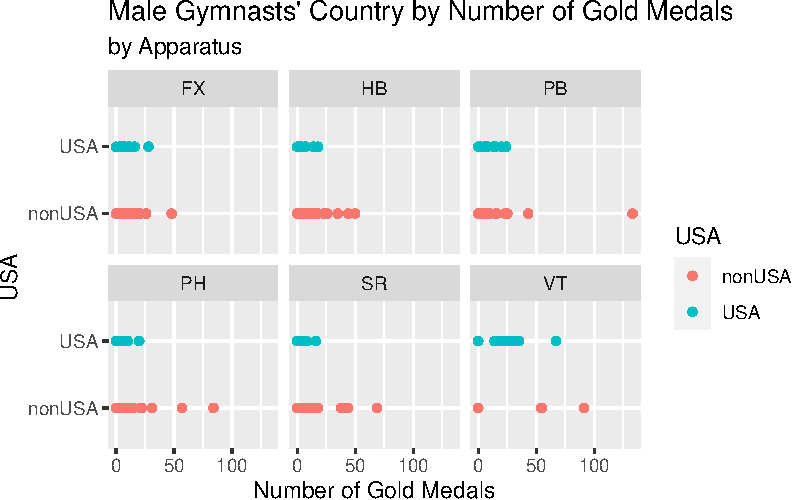
\includegraphics{Main_files/figure-pdf/unnamed-chunk-6-1.pdf}

}

\end{figure}

\begin{Shaded}
\begin{Highlighting}[]
\NormalTok{number\_athletes }\SpecialCharTok{|\textgreater{}}
  \FunctionTok{filter}\NormalTok{(Round }\SpecialCharTok{==} \StringTok{"AAfinal"}\NormalTok{) }\SpecialCharTok{|\textgreater{}}
  \FunctionTok{ggplot}\NormalTok{(}\FunctionTok{aes}\NormalTok{(}\AttributeTok{x =}\NormalTok{ athletes\_participated)) }\SpecialCharTok{+}
    \FunctionTok{geom\_histogram}\NormalTok{() }\SpecialCharTok{+}
    \FunctionTok{labs}\NormalTok{(}\AttributeTok{x =} \StringTok{"Number of Unique Athletes Competed"}\NormalTok{,}
         \AttributeTok{y =} \StringTok{"Frequency"}\NormalTok{,}
         \AttributeTok{title =} \StringTok{"Distribution of Athletes Competed at AA Finals"}\NormalTok{)}
\end{Highlighting}
\end{Shaded}

\begin{verbatim}
`stat_bin()` using `bins = 30`. Pick better value with `binwidth`.
\end{verbatim}

\begin{figure}[H]

{\centering 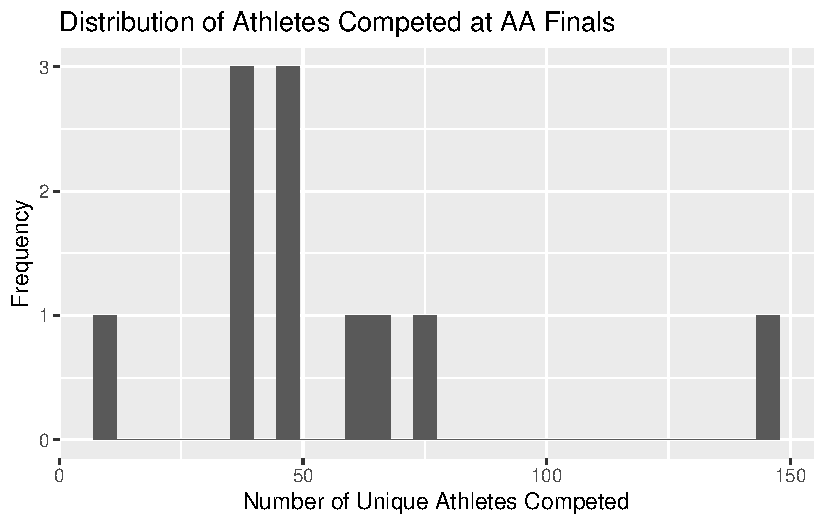
\includegraphics{Main_files/figure-pdf/unnamed-chunk-6-2.pdf}

}

\end{figure}

\begin{Shaded}
\begin{Highlighting}[]
\NormalTok{number\_athletes }\SpecialCharTok{|\textgreater{}}
  \FunctionTok{filter}\NormalTok{(Round }\SpecialCharTok{==} \StringTok{"final"}\NormalTok{) }\SpecialCharTok{|\textgreater{}}
  \FunctionTok{ggplot}\NormalTok{(}\FunctionTok{aes}\NormalTok{(}\AttributeTok{x =}\NormalTok{ athletes\_participated)) }\SpecialCharTok{+}
    \FunctionTok{geom\_histogram}\NormalTok{() }\SpecialCharTok{+}
    \FunctionTok{facet\_wrap}\NormalTok{(}\SpecialCharTok{\textasciitilde{}}\NormalTok{ Round) }\SpecialCharTok{+}
    \FunctionTok{labs}\NormalTok{(}\AttributeTok{x =} \StringTok{"Number of Unique Athletes Competed"}\NormalTok{,}
         \AttributeTok{y =} \StringTok{"Frequency"}\NormalTok{,}
         \AttributeTok{title =} \StringTok{"Distribution of Athletes Competed at Final Rounds"}\NormalTok{,}
         \AttributeTok{subtitle =} \StringTok{"Individual Apparatuses"}\NormalTok{)}
\end{Highlighting}
\end{Shaded}

\begin{verbatim}
`stat_bin()` using `bins = 30`. Pick better value with `binwidth`.
\end{verbatim}

\begin{figure}[H]

{\centering 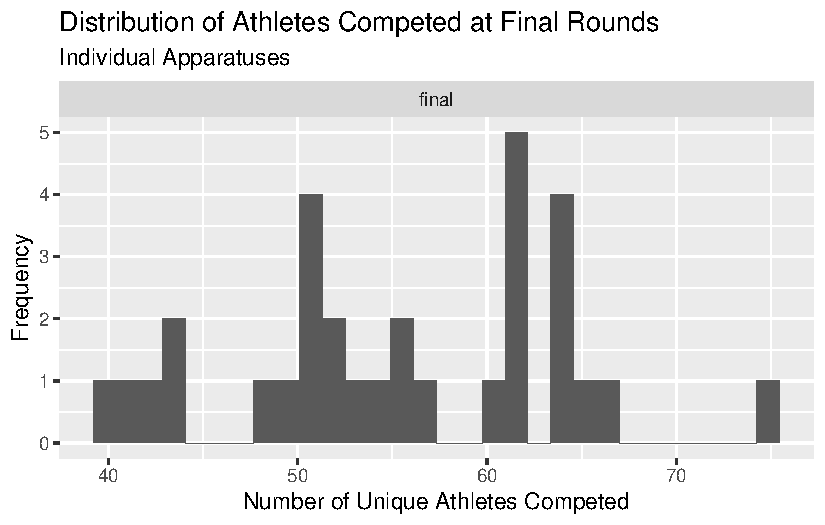
\includegraphics{Main_files/figure-pdf/unnamed-chunk-6-3.pdf}

}

\end{figure}

\begin{Shaded}
\begin{Highlighting}[]
\FunctionTok{ggplot}\NormalTok{(number\_athletes, }\FunctionTok{aes}\NormalTok{(}\AttributeTok{x =}\NormalTok{ athletes\_participated)) }\SpecialCharTok{+}
  \FunctionTok{geom\_histogram}\NormalTok{() }\SpecialCharTok{+}
  \FunctionTok{labs}\NormalTok{(}\AttributeTok{x =} \StringTok{"Number of Unique Athletes Competed"}\NormalTok{,}
       \AttributeTok{y =} \StringTok{"Frequency"}\NormalTok{,}
       \AttributeTok{title =} \StringTok{"Distribution of Athletes Competed at Competitions"}\NormalTok{)}
\end{Highlighting}
\end{Shaded}

\begin{verbatim}
`stat_bin()` using `bins = 30`. Pick better value with `binwidth`.
\end{verbatim}

\begin{figure}[H]

{\centering 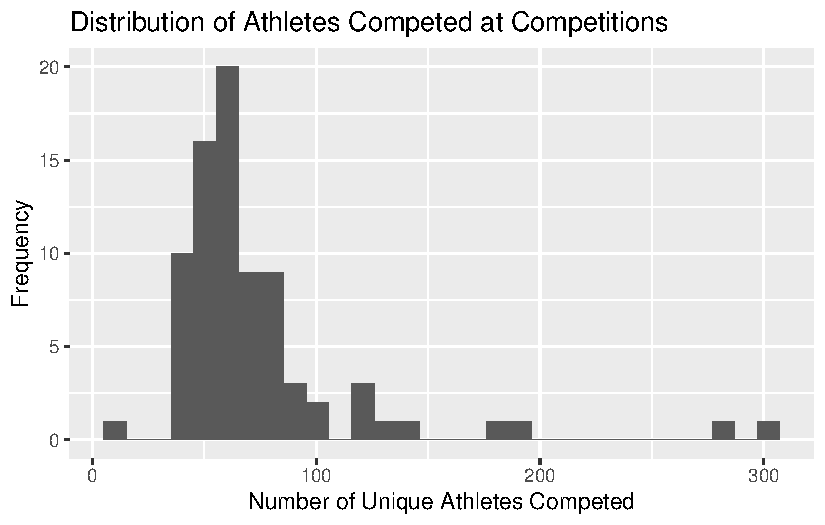
\includegraphics{Main_files/figure-pdf/unnamed-chunk-6-4.pdf}

}

\end{figure}



\end{document}
